\subsection{Boosted Top Tagging}
\label{subsec:sel_toptag_boosted}

Jet substructure techniques can be used to identify boosted top decays where all the decay products are contained within a single jet. Wider jets are considered so that substructure methods are applicable for tops with moderate boost. In this analysis, jets with $R=1.5$ are considered so that tops with $\pt>250\:\GeV$ are fairly well contained within the jet. Soft drop jet grooming, $N$-subjettiness, and subjet $\Bot$-tagging are applied to tag top decays.

By analyzing the radiation pattern within a jet, it is possible to differentiate between a jet induced by a single parton and a jet induced by the decay of a massive particle. The soft drop algorithm removes soft, wide angled radiation and decomposes a jet into subjets that correspond to the underlying hard partons that induce the jet. The settings used for soft drop are $\beta=0$ and $z_{\mbox{\scriptsize{cut}}}=0.1$. The soft drop mass ($M_{\mbox{\scriptsize{soft drop}}}$) spectrum is shown in Fig.~\ref{fig:softdrop}, for events with a single ``Tight'' muon or electron, $M_T>160\:\GeV$, and at least one AK4CHS $\Bot$-tagged jet.

\begin{figure}[htbp]
  \centering
  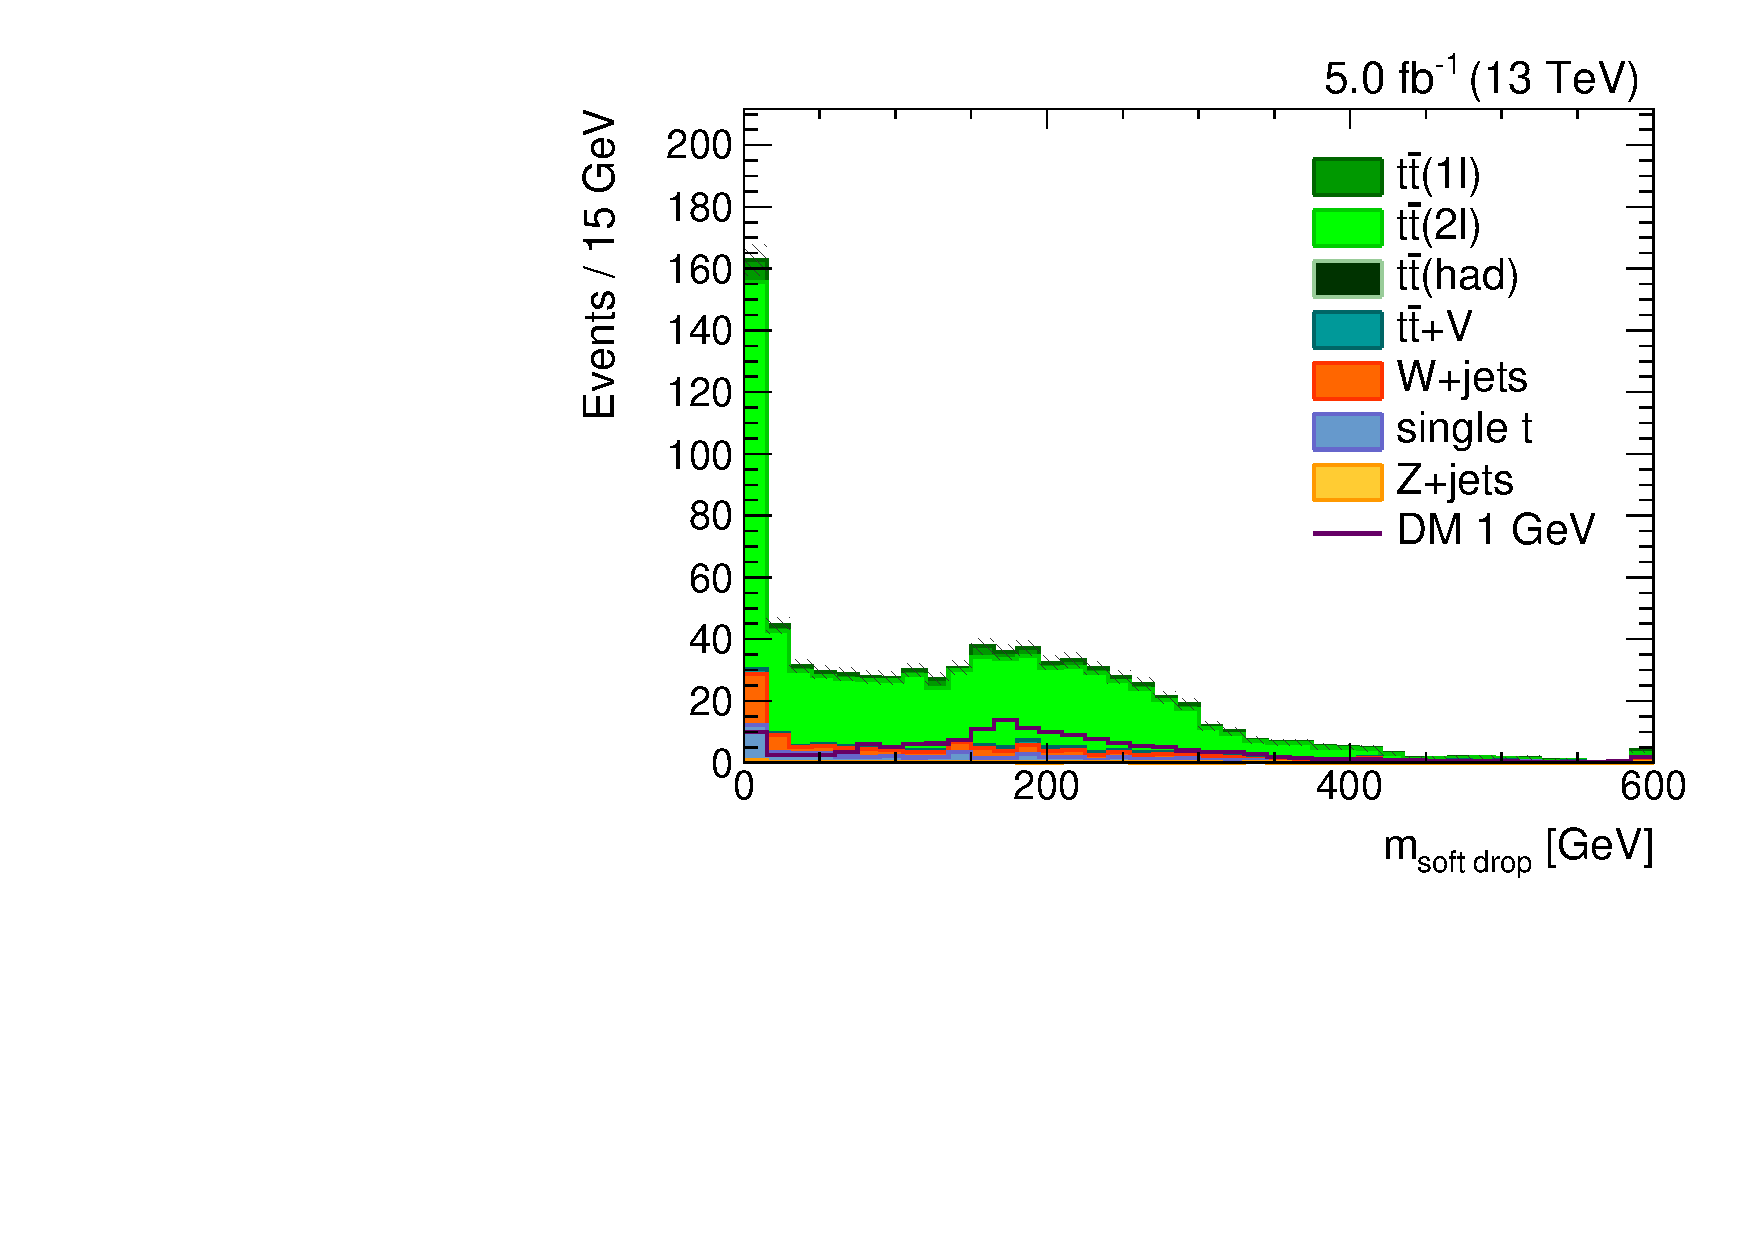
\includegraphics[width=0.48\textwidth]{figures/softdrop.pdf}
  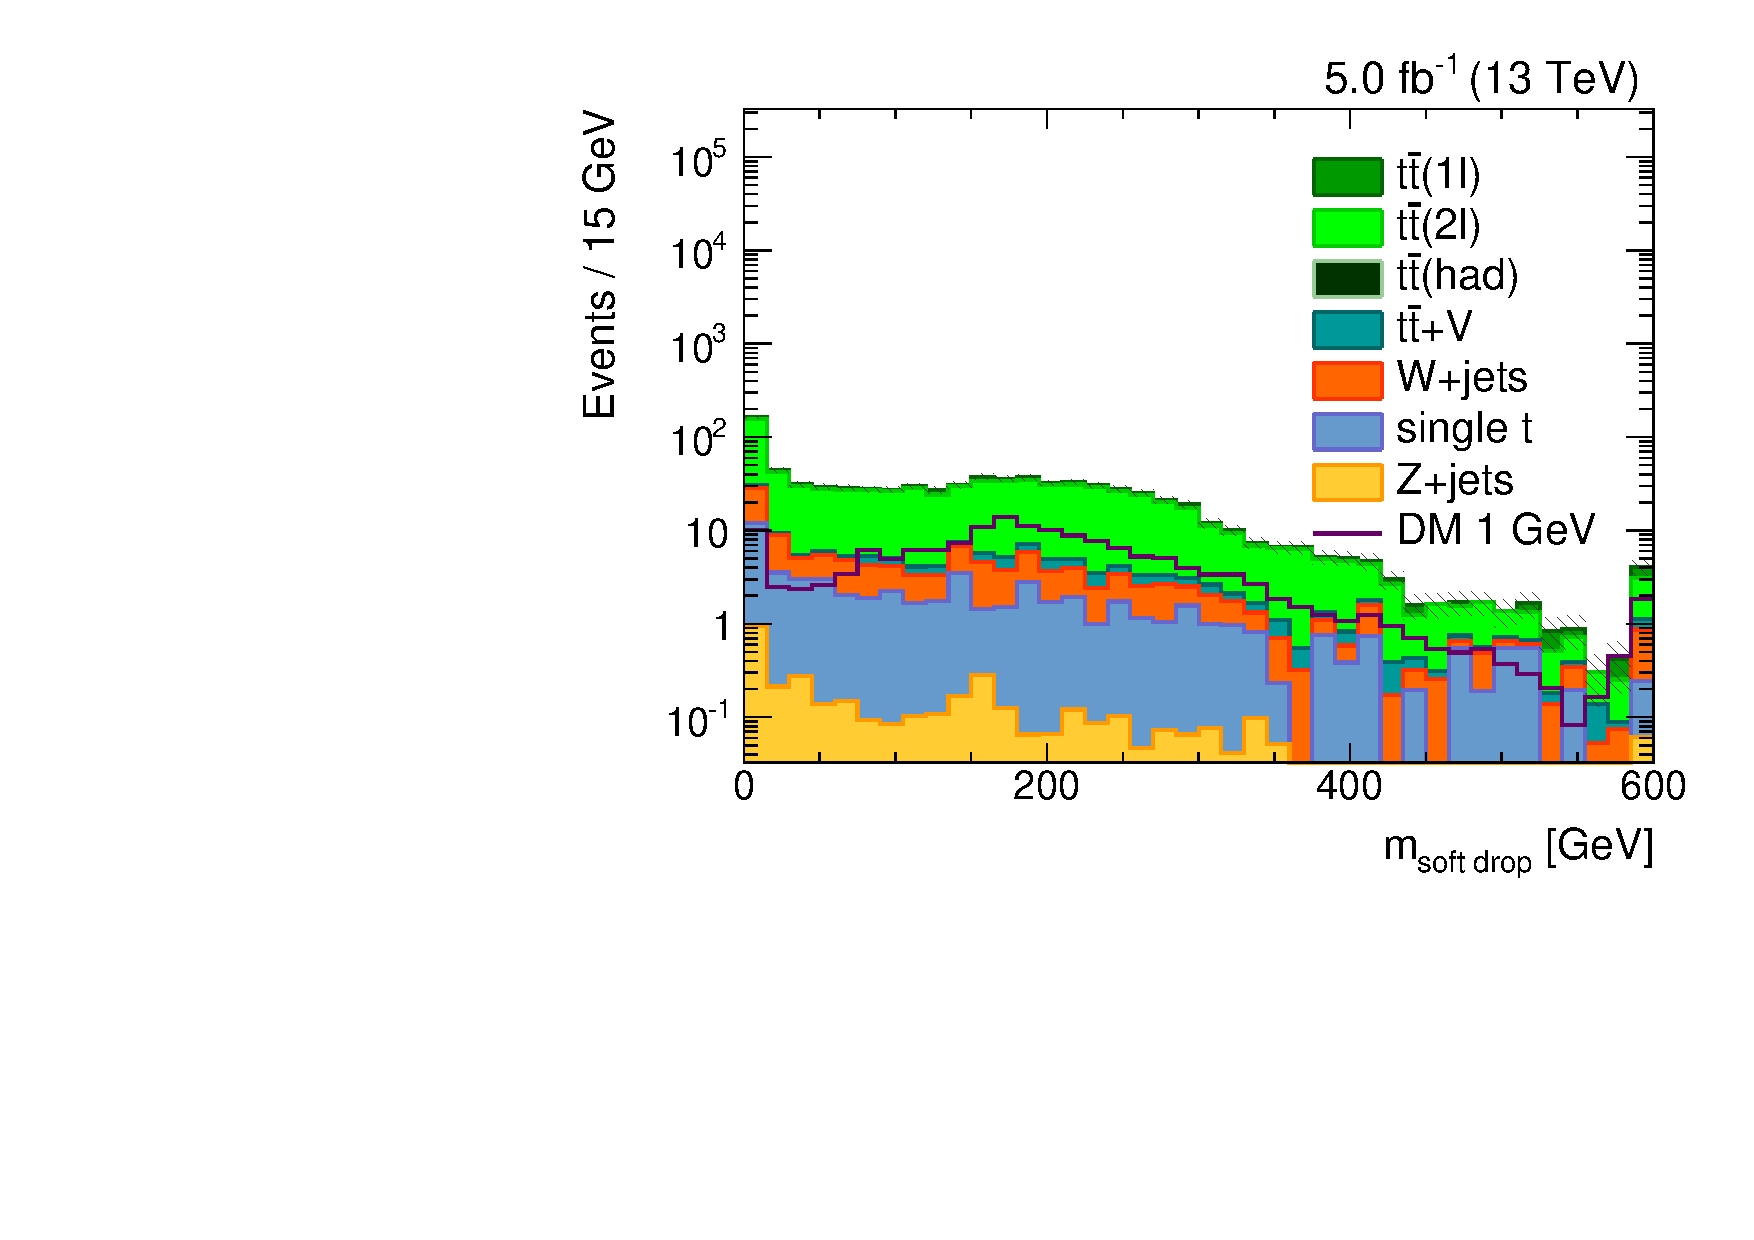
\includegraphics[width=0.48\textwidth]{figures/softdroplog.pdf}
  \caption{Jet mass distribution after grooming with the soft drop ($\beta=0, z_{\mbox{\scriptsize{cut}}}=0.1$) algorithm.}
  \label{fig:softdrop}
\end{figure}

$N$-subjettiness quantifies the likelihood a jet comprises of $N$ or more prongs. The discriminating variable is the ratio of $N$-subjettiness quantities; in particular, the $\tau_n/\tau_{n-1}$ ratio quantifies the likelihood the jet comprises of $n$ prongs. Hence, $\tau_3/\tau_2$ is used to help identify top decays. The $\tau_3/\tau_2$ distribution for events with $M_{\mbox{\scriptsize{soft drop}}}>75\:\GeV$ is shown in Fig.~\ref{fig:tau32}.

\begin{figure}[htbp]
  \centering
  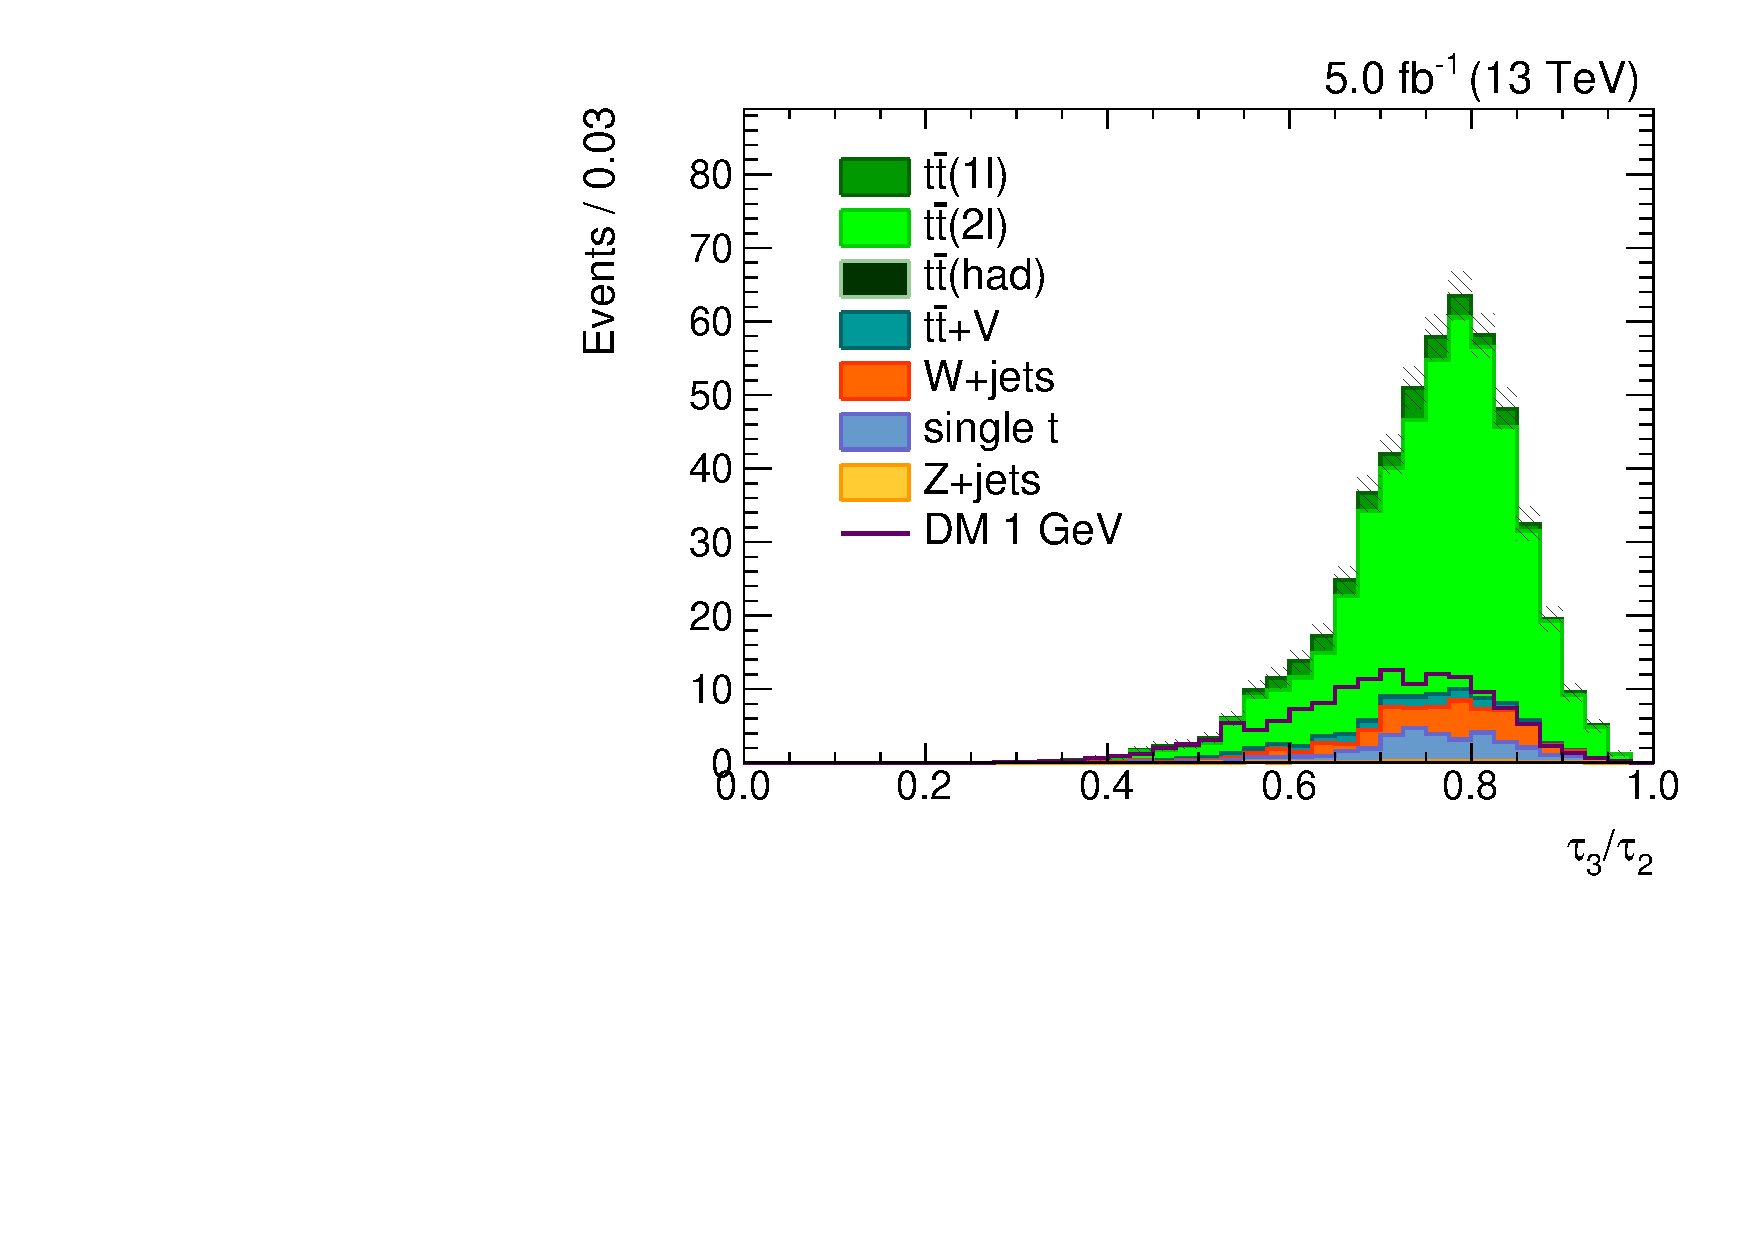
\includegraphics[width=0.48\textwidth]{figures/tau32.pdf}
  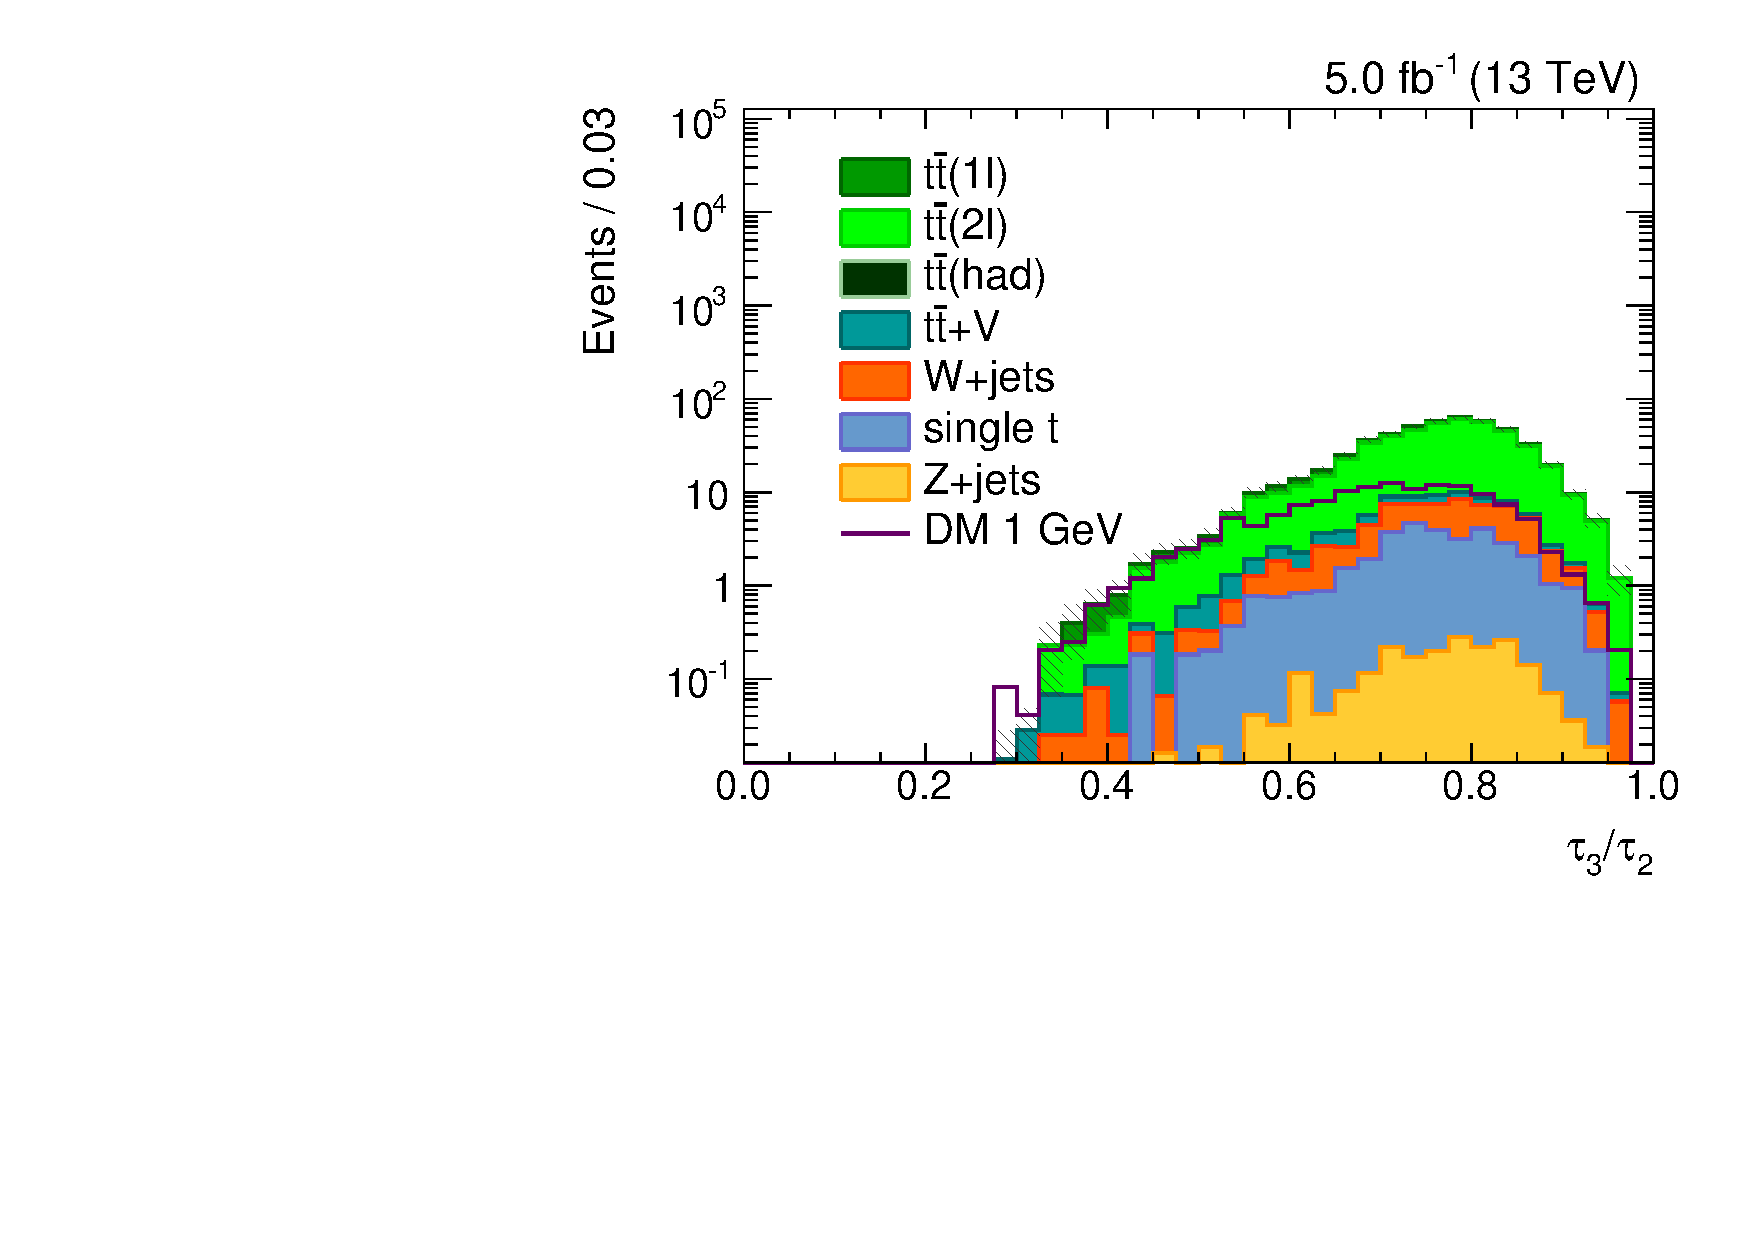
\includegraphics[width=0.48\textwidth]{figures/tau32log.pdf}
  \caption{Distribution of $\tau_3/\tau2$ for jets with $M_{\mbox{\scriptsize{soft drop}}}>75\:\GeV$.}
  \label{fig:tau32}
\end{figure}

The $\Bot$ quark from the top decay is expected to be contained in the wide jet and therefore the corresponding subjet should have properties similar to typical $\Bot$-jets. The CSVv2+IVF $\Bot$-tag algorithm is performed on subjets from the soft drop decomposition to provide further discrimination for top decays. The distribution for the largest $\Bot$-tag value among subjets in a jet, for jets with $M_{\mbox{\scriptsize{soft drop}}}>75\:\GeV$, is shown in Fig.~\ref{fig:subjet_btag}.

\begin{figure}[htbp]
  \centering
  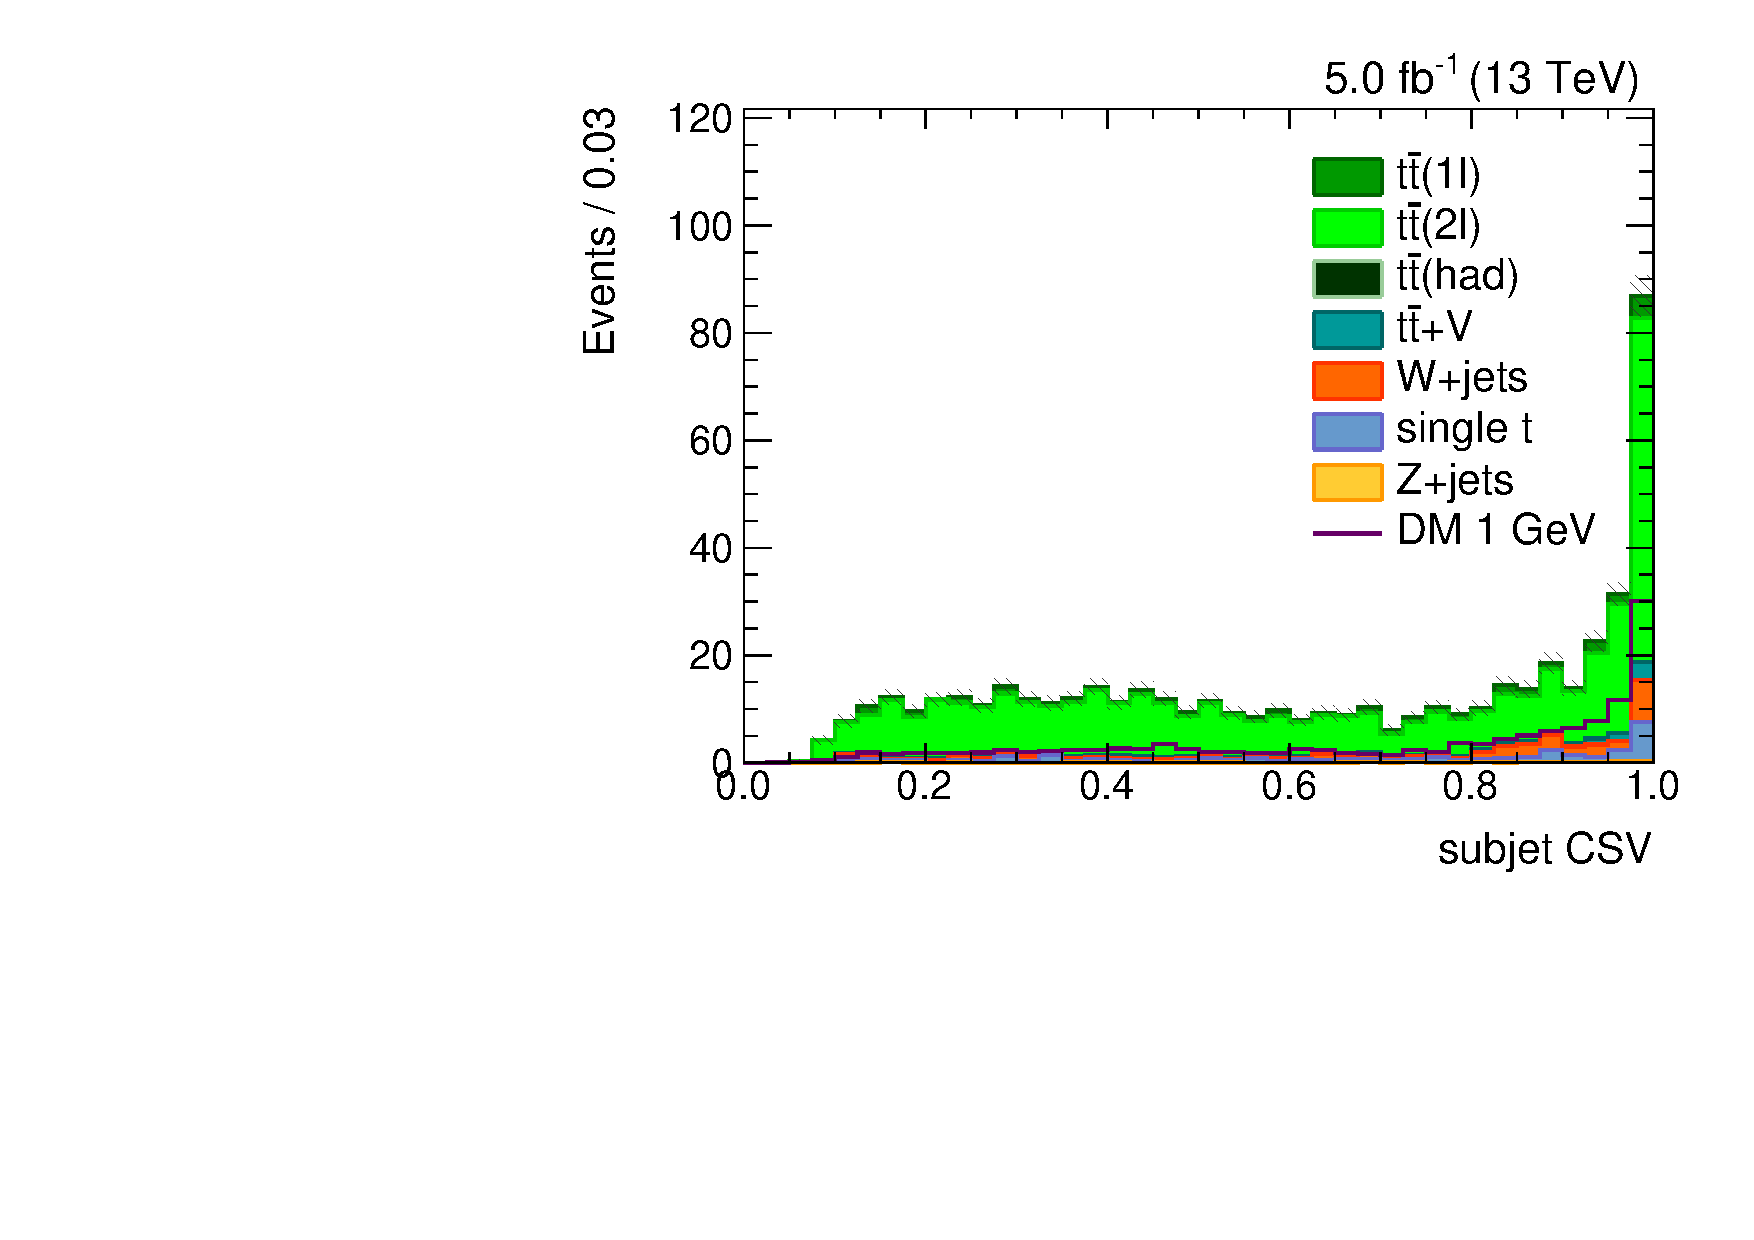
\includegraphics[width=0.48\textwidth]{figures/subjetbtag.pdf}
  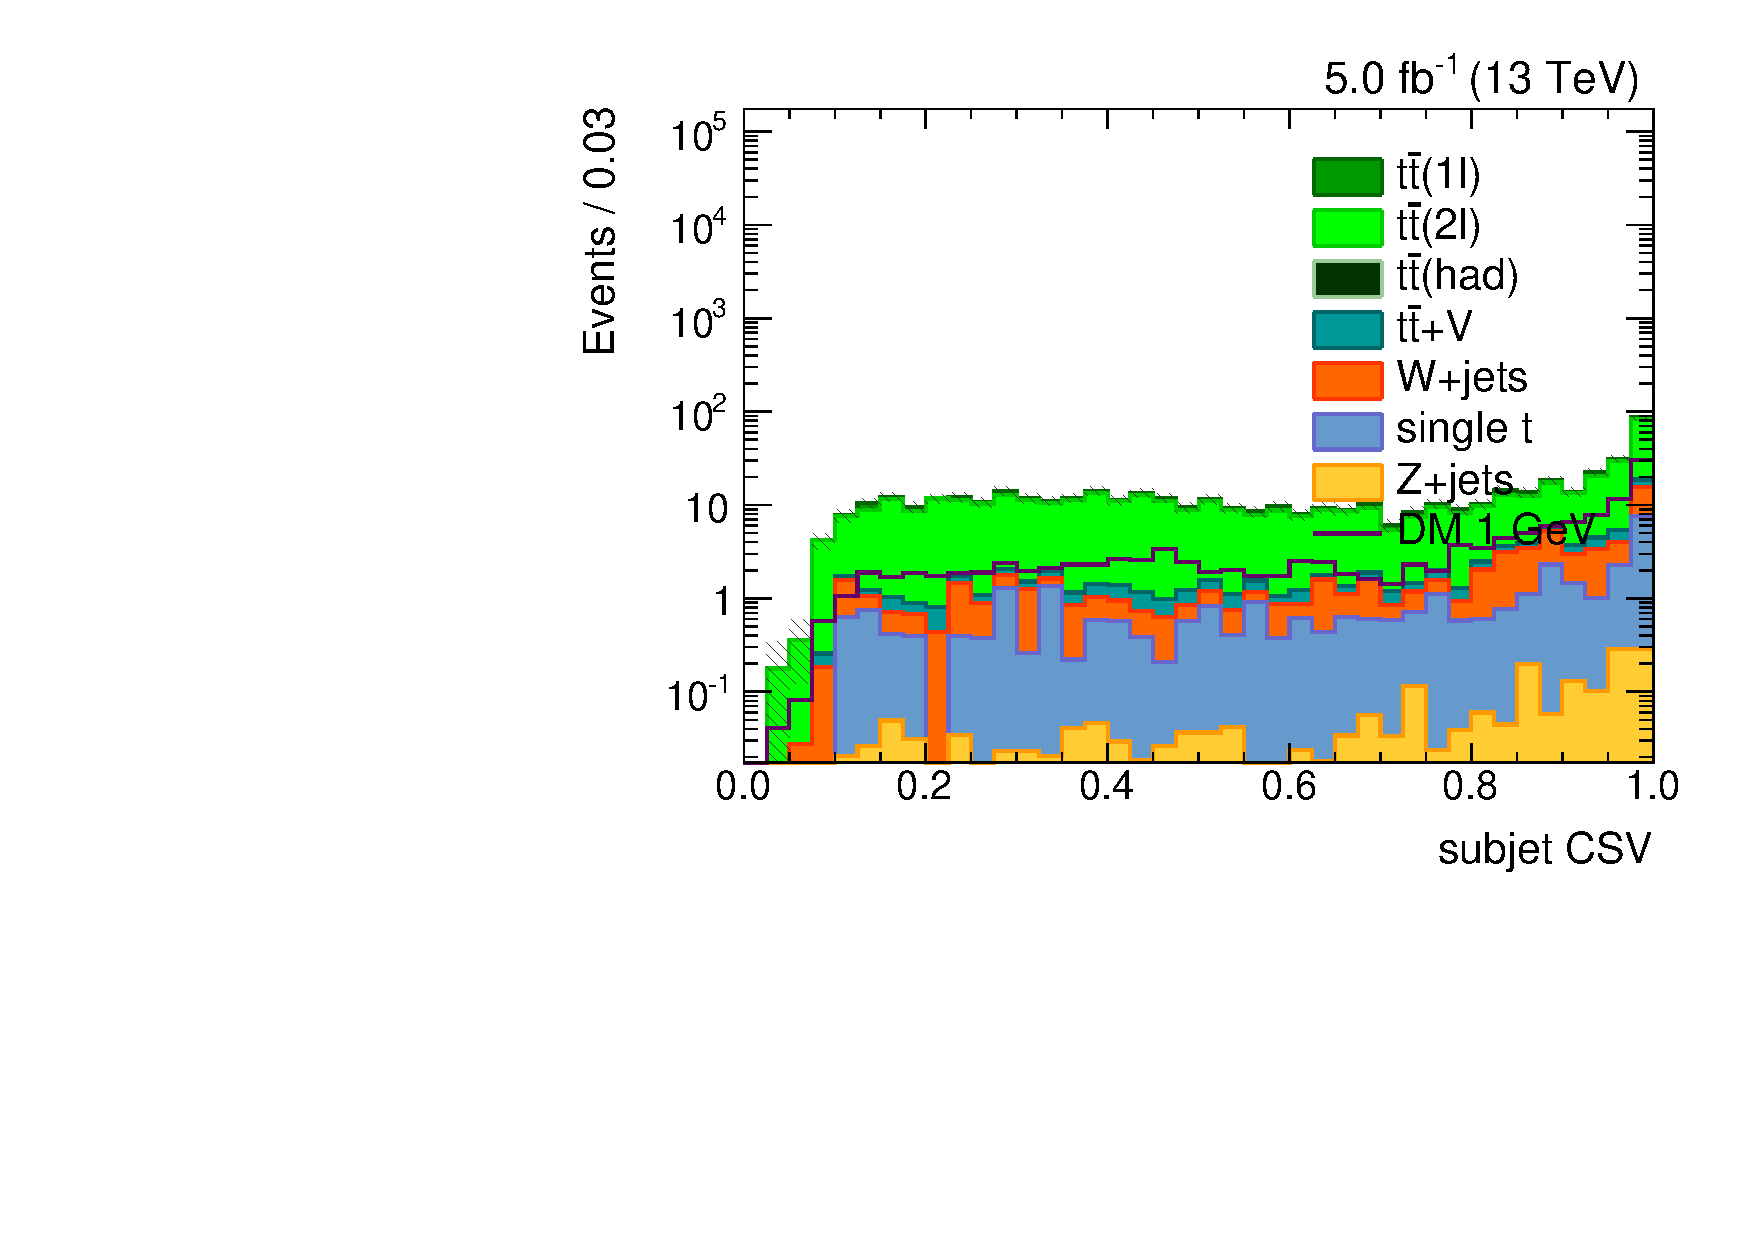
\includegraphics[width=0.48\textwidth]{figures/subjetbtaglog.pdf}
  \caption{Distribution of the largest CSVv2+IVF value among subjets in a wide jet. The wide jet must have $M_{\mbox{\scriptsize{soft drop}}}>75\:\GeV$.}
  \label{fig:subjet_btag}
\end{figure}

A boosted top is identified by the following requirements, 
\begin{itemize}
\item CA15CHS jet with $\pt>250\:\GeV$ and $|\eta|<2.4$,
\item $M_{\mbox{\scriptsize{soft drop}}} > 75\:\GeV$
\item $\tau_3/\tau_2 < 0.75$
\item maximum subjet $\Bot$-tag $> 0.4$
\end{itemize}
